\documentclass{article}

\usepackage{amsmath}
\usepackage{amssymb}
\usepackage{enumerate}
\usepackage[spanish]{babel}
\usepackage{cancel}
\usepackage{caption}
\usepackage[margin=1.5in]{geometry}
\usepackage{graphicx}
\usepackage[utf8]{inputenc}
\usepackage{tcolorbox}
\usepackage{esint}
\usepackage{hyperref}
\hypersetup{
    colorlinks,
    citecolor=black,
    filecolor=black,
    linkcolor=black,
    urlcolor=black,
}

\renewcommand{\Bbb}{\mathbb}

\tcbuselibrary{theorems}

\title{Apuntes teórico-prácticos de Física I A (62.01) \\ Cátedra Menikheim \\ 1° C 2004}
\author{Darío Eduardo Ramos}

\definecolor{ududff}{rgb}{0.30196078431372547,0.30196078431372547,1}
\definecolor{cqcqcq}{rgb}{0.7529411764705882,0.7529411764705882,0.7529411764705882}

\begin{document}
\maketitle

\tableofcontents{}
\newpage

\section{Cinemática}

\subsection{Definiciones iniciales}

La \textbf{cinemática} es la rama de la física que describe el movimiento de los objetos sólidos sin considerar las causas que lo originan. 

El primer \textbf{modelo} que se adoptará para los cuerpos físicos a modelar será el de \textbf{punto material o partícula}: dichos cuerpos físicos serán considerados como sin volumen, pero sí con masa. Toda esa masa estará ``concentrada'' en el centro de masa del cuerpo, que será el punto que represente al objeto.

\textbf{Movimiento}: Un cuerpo será considerado en movimiento cuando cambie de posición a lo largo del tiempo respecto a un sistema de referencia considerado fijo o inercial. Más sobre esto último cuando se estudien los sistemas inerciales y no inerciales.

Cuando el cuerpo se desplaza desde una posición inicial dada por el vector $\overrightarrow{ r_i }$ a una posición final dada por el vector $\overrightarrow{ r_f }$, en un tiempo $\Delta t$, se definen las siguientes magnitudes vectoriales y escalares:

\begin{itemize}
\item \textbf{Vector desplazamiento:} $\overrightarrow{ \Delta r } = \overrightarrow{r_f} - \overrightarrow{r_i}$. Por como está definido, el vector $\overrightarrow{\Delta r}$ va de $\overrightarrow{r_i}$ hacia $\overrightarrow{r_f}$.
\item \textbf{Camino recorrido (escalar):}  $\Delta s$ = longitud del arco de trayectoria entre posición inicial y final.
\item \textbf{Vector velocidad media:} $\overrightarrow{v_m} = \frac{\overrightarrow{\Delta r}}{\Delta t}$
\item \textbf{Rapidez media (escalar):} $\overline{v} = \frac{\Delta s}{\Delta t}$
\item \textbf{Vector velocidad instantánea:}

\begin{equation}
\tcboxmath[colback=orange!25!white,colframe=orange]{
\overrightarrow{v} = \lim_{\Delta t \rightarrow 0} \frac{ \mathop{\overrightarrow{\Delta r}} }{\Delta t} = \frac{d\overrightarrow{r}}{\mathop{dt}}
}
\end{equation}

Nótese entonces que la velocidad instantánea es la derivada de la posición respecto al tiempo. Además, al ser $\overrightarrow{r}(t)$ una función vectorial del tiempo, $\overrightarrow{v}$ también lo es. Punto a punto, el vector $\overrightarrow{v}(t_0)$ es tangente a la curva de la trayectoria en el punto $\overrightarrow{r}(t_0)$ y su sentido es el del movimiento.
\item \textbf{Rapidez instantánea:}

\begin{equation}
v = \lim_{\Delta t \rightarrow 0} \frac{\Delta s}{\Delta t} = \frac{\mathop{ds}}{\mathop{dt}}
\end{equation}

\item \textbf{Vectores aceleración media e instantánea:}

\begin{equation}
\overrightarrow{a_m} = \frac{ \overrightarrow{ \Delta v } }{ \Delta t }
\end{equation}

\begin{equation}
\tcboxmath[colback=orange!25!white,colframe=orange]{
\overrightarrow{a} = \lim_{\Delta t \rightarrow 0} \frac{ \overrightarrow{ \Delta v } }{\Delta t} = \frac{ \mathop{d\overrightarrow{v}} }{ \mathop{dt} } = \frac{ \mathop{ d^2 \overrightarrow{r} } }{ \mathop{ dt^2 } }
}
\end{equation}

Cualquier cambio en el sentido, dirección o norma del vector velocidad indica que existe aceleración. Esto implica que en todo movimiento curvo hay aceleración no nula.

\end{itemize}

\subsection{Movimiento circular y movimiento curvo en general}

\subsubsection{Movimiento circular}

Algunas definiciones iniciales:

\begin{itemize}
\item \textbf{Velocidad angular (escalar):} $\omega = \frac{ \mathop{d\alpha} }{dt}$ = derivada del ángulo en función del tiempo.
\item \textbf{Ángulo en función del tiempo:} $\Delta \alpha = \omega \Delta t$
\item \textbf{Radianes:} $\alpha_{\mathop{rad}} = \frac{\text{longitud de arco}}{ \text{radio} }$
\item Relación entre $\omega$, el radio y la rapidez instantánea:

\begin{equation}
\alpha_{\mathop{rad}} = \frac{\text{longitud de arco}}{ \text{radio} } \Rightarrow \Delta \alpha = \frac{ \Delta s } {R} \Leftrightarrow \Delta s = \mathop{\Delta\alpha} \cdot R
\end{equation}

Reemplazando en la expresión general de la rapidez media:

\begin{equation}
\overline{v} = \frac{\Delta s}{\Delta t} \Rightarrow \overline{v} = \frac{\mathop{\Delta\alpha} \cdot R}{\Delta t} \Rightarrow v = \lim_{\Delta t \rightarrow 0} \underbrace{ \frac{\Delta \alpha}{\Delta t} }_{\omega} R \Rightarrow \tcboxmath[colback=orange!25!white,colframe=orange]
{ v = \omega R }
\end{equation}

De esta igualdad se puede concluir que si $\omega$ es constante, la rapidez instantánea también. Esto no aplica al vector velocidad, que tendrá norma constante, pero dirección variable.
\end{itemize}

\subsubsection{El vector velocidad}

Considerando $\overrightarrow{\omega}$ como un vector perpendicular, instante a instante, al plano del movimiento, se puede demostrar que para todo movimiento circular:

\begin{equation}
\tcboxmath[colback=orange!25!white,colframe=orange]{
\overrightarrow{v} = \overrightarrow{\omega} \times \overrightarrow{r}
}
\end{equation}

En esta igualdad, $\overrightarrow{r}$ es el vector posición. Dado que el sistema de referencia puede ser cartesiano o intrínseco, en ambos casos $\overrightarrow{r}$ se relaciona con el radio, aunque su expresión sea diferente.

Recuérdese que el vector resultado del producto vectorial es ortogonal a ambos vectores multiplicados a la vez. En este caso, $\overrightarrow{v}$ es ortogonal a $\overrightarrow{\omega}$ y también es ortogonal a $\overrightarrow{r}$. Además, el sentido de $\overrightarrow{v}$ está dado por la regla de la mano derecha.

\subsubsection{Coordenadas intrínsecas}

\begin{figure}[ht]
\centering
\caption{Coordenadas intrínsecas}
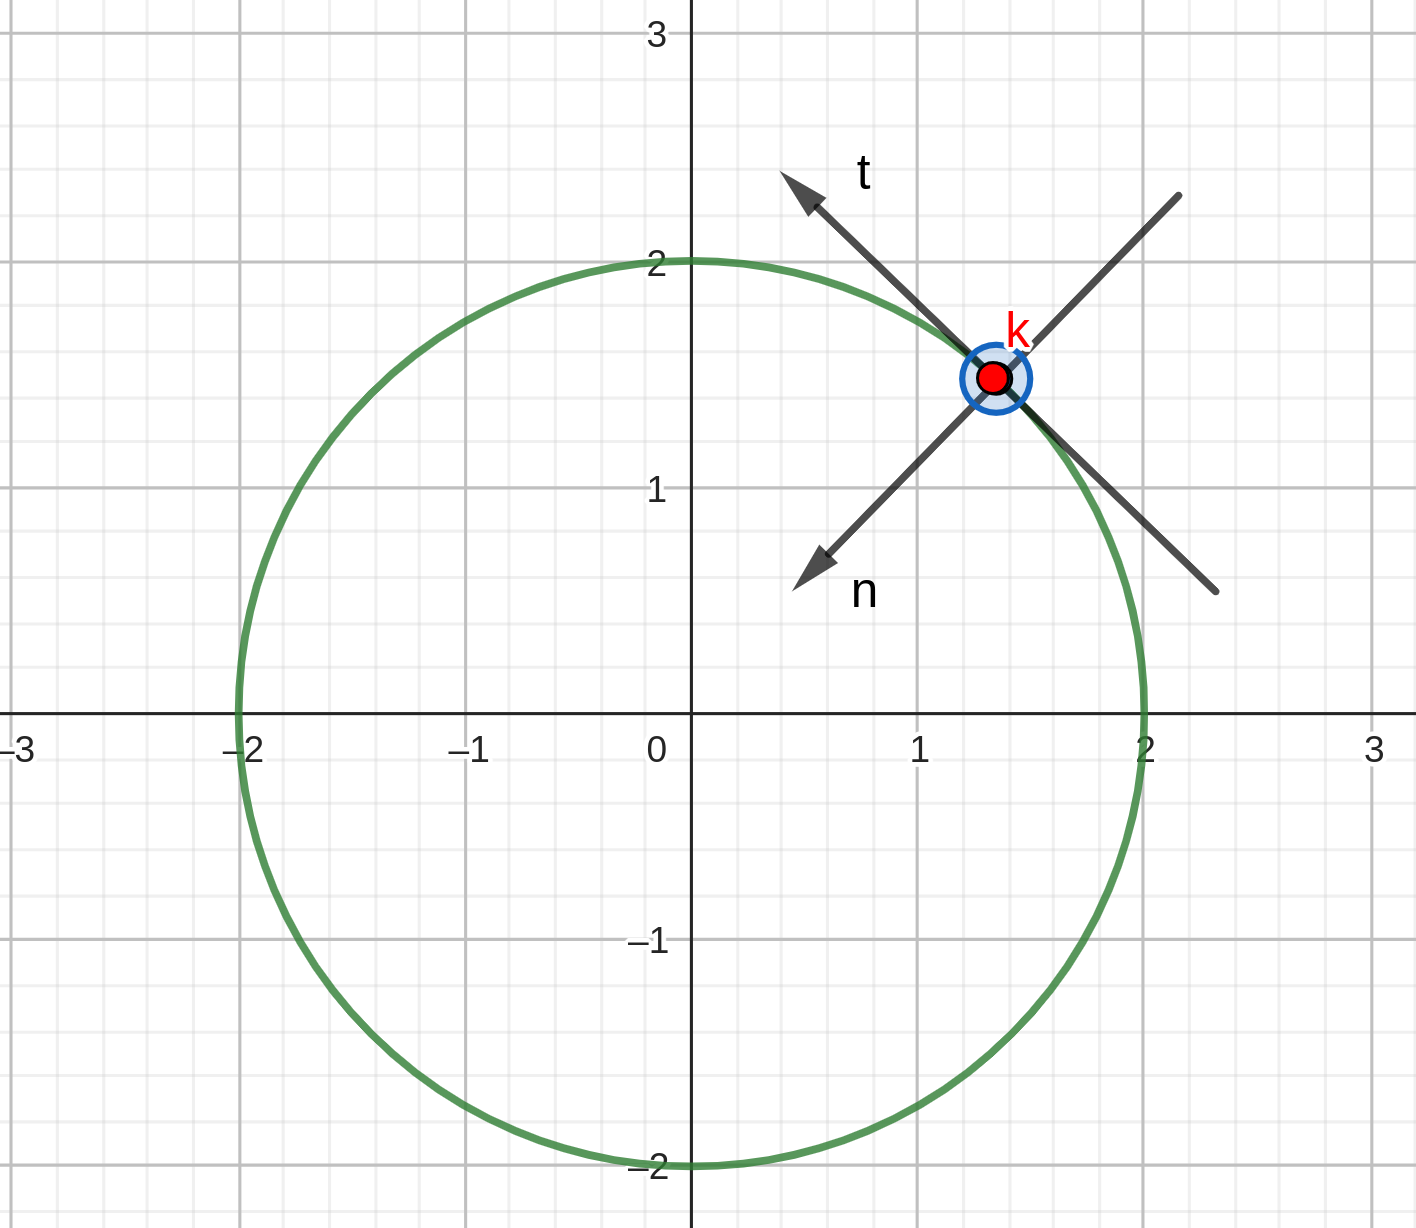
\includegraphics[scale=1]{../../common/img/62.01/theory/01-kinematics-intrinsic-coords.png}
\label{fig:intrinsicCoords}
\end{figure}

Obsérvese la figura \ref{fig:intrinsicCoords}. Para un instante determinado, el eje tangente $t$ se define positivo en el sentido de la velocidad. En cuanto al eje normal $n$, es positivo en el sentido de la concavidad, o sea hacia la parte interior del círculo. Finalmente, el eje binormal $k$, es positivo en el sentido de la aceleración angular $\gamma$. Es importante entender que este sistema de referencia es relativo a un instante específico de tiempo: para cada instante de tiempo, los ejes serán diferentes.

Con esta terna de ejes, resulta, si se denotan el radio del círculo con $R$, y los versores de los ejes con $\check{t}$, $\check{n}$ y $\check{k}$:

\begin{subequations}
\begin{align}
\overrightarrow{r} &= -R \check{n} \\
\overrightarrow{v} &= \omega R \check{t} \\
\overrightarrow{a_{\mathop{tg}}} &= \pm \gamma R \check{t} \\
\overrightarrow{a_{n}} &= \omega v \check{n}
\end{align}
\end{subequations}

Además, $R = ||\overrightarrow{r}||$ y $\gamma = ||\overrightarrow{\gamma}||$. Ahora bien, ¿de dónde salieron las expresiones de la aceleración tangencial y la aceleración normal? De derivar la velocidad. Ahora bien, al hacer eso, se utiliza el resultado de que la derivada de un producto vectorial sigue la misma regla que la derivada del producto de funciones. Verbigracia:

\begin{equation}
\overrightarrow{v} = \overrightarrow{\omega} \times \overrightarrow{r} \wedge \overrightarrow{a} = \frac{\mathop{d\overrightarrow{v}}}{\mathop{dt}} \Rightarrow \overrightarrow{a} = \underbrace{ \frac{\mathop{d\overrightarrow{\omega}}}{\mathop{dt}} }_{\overrightarrow{\gamma}} \times \overrightarrow{r} + \overrightarrow{\omega} \times \underbrace{ \frac{\mathop{d\overrightarrow{r}}}{\mathop{dt}} }_{\overrightarrow{v}}
\end{equation}

Resulta entonces:

\begin{equation}
\tcboxmath[colback=orange!25!white,colframe=orange, title=acelerac. en mov. circ.]{
\overrightarrow{a} = \underbrace{ \overrightarrow{\gamma} \times \overrightarrow{r} }_{\overrightarrow{a_{\mathop{tg}}}} + \underbrace{ \overrightarrow{\omega} \times \overrightarrow{v} }_{\overrightarrow{a_n}}
}
\end{equation}

En un movimiento circular, tanto $\overrightarrow{\omega}$ como $\overrightarrow{\gamma}$ jamás cambian su dirección, aunque sí puede cambiar su norma o su sentido.

Dado que $\overrightarrow{a_n}$ suele ser de especial interés por estar asociada a las fuerzas centrífugas, es de interés su norma:

\begin{equation}
a_n = ||\overrightarrow{a_n}|| = \omega v = \omega^2 R = \frac{v^2}{R}
\end{equation}

\subsubsection{Movimiento curvo generalizado}

Todo movimiento curvo puede ser analizado como la unión de movimiento circulares instantáneos, donde el radio es variable. Además, pasa a llamarse \textbf{radio de curvatura} y se denota con la letra $\rho$. Utilizando coordenadas intrínsecas, resulta:

\begin{equation}
\tcboxmath[colback=orange!25!white,colframe=orange]{
\overrightarrow{v} = \omega \rho \check{t}
}
\end{equation}

\begin{equation}
\tcboxmath[colback=orange!25!white,colframe=orange]{
\overrightarrow{a} = \underbrace{ \pm \gamma \rho \check{t} }_{\overrightarrow{a_{\mathop{tg}}}} + \underbrace{ \omega v \check{n} }_{\overrightarrow{a_n}}
}
\end{equation}

En este escenario generalizado, $\rho$ debe deducirse geométricamente, aunque esa no es la única forma de calcularlo. Por otro lado, puede decirse que $\overrightarrow{a_{\mathop{tg}}}$ está asociado a cambios en la norma de $\overrightarrow{v}$, en tanto $\overrightarrow{a_n}$ está asociado a cambios de dirección. 

\end{document}